% fig:uldlgrants — layout provided by author (clean UL/DL asymmetry).
\begin{tikzpicture}[
    font=\sffamily,
    block/.style={rectangle, draw=black!40, rounded corners=3pt, align=center, inner sep=2.5pt, font=\fontsize{9.8}{11.5}\selectfont},
    comp/.style={rectangle, draw=black!40, rounded corners=3pt, align=center, fill=grey_box, inner sep=2.5pt, font=\fontsize{9.8}{11.5}\selectfont},
    title/.style={anchor=north west, font=\fontsize{12.7}{15}\selectfont\bfseries, inner sep=0pt},
    subtitle/.style={anchor=north west, font=\fontsize{9.8}{12.1}\selectfont, text=grey_text, inner sep=0pt},
    arrow/.style={-Latex, thick, shorten >=2pt, shorten <=2pt},
    dashed_arrow/.style={-Latex, thick, dashed, grey_text, shorten >=2pt, shorten <=2pt}
]

% ============================================================
% SECTION (a) - Uplink
% ============================================================

\node[title] (titleA) at (0, 10) {(a) Uplink scheduling (UE must request)};
\node[subtitle] (subA) at (0, 9.5) {UEs must request resources. Scheduler allocates limited UL PRBs.};

\node[anchor=west, align=center] (uav_tele) at (0.15, 8.2) {%
  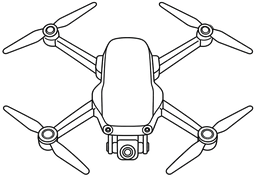
\includegraphics[height=0.60cm]{uav}\\[1.5pt]%
  \color{uav_color}\fontsize{11.5}{13.5}\selectfont\bfseries UAV UE\\[-2pt]%
  \color{uav_color}\fontsize{9.2}{10.9}\selectfont(telemetry)%
};
\node[block, fill=uav_color!12, draw=uav_color!60] (uav_bsr) at (5.35, 8.2) {%
  \bfseries SR / BSR\\[-1pt]%
  \fontsize{8.6}{10.4}\selectfont indicates demand\\[-2pt]%
  \fontsize{8.6}{10.4}\selectfont and buffer status%
};
\draw[arrow, uav_color] (uav_tele.east) -- (uav_bsr.west);

\node[anchor=west, align=center] (co_tenant_video) at (0.15, 6.15) {%
  
\includegraphics[height=0.72cm]{ues_rogues}\\[1.5pt]%
  \color{video_color}\fontsize{11.5}{13.5}\selectfont\bfseries Co-tenant UE\\[-2pt]%
  \color{video_color}\fontsize{9.2}{10.9}\selectfont(competing traffic)%
};
\node[block, fill=video_color!12, draw=video_color!60] (video_bsr) at (5.35, 6.15) {%
  \bfseries SR / BSR\\[-1pt]%
  \fontsize{8.6}{10.4}\selectfont indicates demand\\[-2pt]%
  \fontsize{8.6}{10.4}\selectfont and buffer status%
};
\draw[arrow, video_color] (co_tenant_video.east) -- (video_bsr.west);

\node[comp] (gnb_sched_A) at (8.95, 7.175) {%
  \begin{tabular}{@{}c@{}}
  \bfseries gNB\\[-0.5pt]
  \bfseries Scheduler\\[0.5pt]
  {\fontsize{8.6}{10.4}\selectfont Selects UEs}\\[-0.5pt]
  {\fontsize{8.6}{10.4}\selectfont \& allocates}\\[-0.5pt]
  {\fontsize{8.6}{10.4}\selectfont UL PRBs}%
  \end{tabular}%
};

\draw[arrow, uav_color, dashed] (uav_bsr.east) -- ($(gnb_sched_A.west)+(0,0.32cm)$);
\draw[arrow, video_color, dashed] (video_bsr.east) -- ($(gnb_sched_A.west)-(0,0.32cm)$);

\node[block, fill=uav_color!15, draw=uav_color!60] (ul_grant) at (11.45, 7.175) {%
  \bfseries UL Grant\\[-1pt]%
  \fontsize{9.2}{10.9}\selectfont(DCI)%
};
\draw[arrow, grey_text] (gnb_sched_A.east) -- (ul_grant.west);

% same X and line breaks as PDSCH in panel (b)
\node[anchor=west, align=center, font=\fontsize{9.8}{12.1}\selectfont] (pusch) at (13.35, 7.175) {%
  \bfseries PUSCH\\[-2pt]%
  \fontsize{9.2}{10.9}\selectfont\textbf{(UE transmits)}%
};
\draw[dashed_arrow] (ul_grant.east) -- (pusch.west);

\node[
  rectangle, rounded corners=4pt, fill=yellow_box, draw=yellow_border,
  anchor=north west, inner sep=5pt,
  font=\fontsize{9.8}{11.5}\selectfont
] (comp_box) at (0.2, 5.05) {%
  \begin{tabular}{@{}l@{}}
  \textbf{Competition for limited UL PRBs:}\\[0.35pt]
  More co-tenant demand $\rightarrow$ \textbf{later} (and fewer) opportunities for UAV telemetry.%
  \end{tabular}%
};

\begin{scope}[shift={(16.85, 6.15)}]
  \node[align=center, font=\fontsize{9.8}{11.5}\selectfont\bfseries] at (1.95cm, 3.4cm) {%
    UL resource pool\\[-2pt]%
    \fontsize{8.6}{10.4}\selectfont(TDD UL slots)%
  };

  \draw[grey_border, step=0.3cm] (0,0) grid (3.9cm, 3.0cm);
  \draw[thick, black!50] (0,0) rectangle (3.9cm, 3.0cm);

  \node[grey_text, left=2pt, font=\fontsize{8.6}{10.4}\selectfont] at (0, 0) {PRB 0};
  \node[grey_text, left=2pt, font=\fontsize{8.6}{10.4}\selectfont] at (0, 3.0cm) {PRB 9};
  \node[grey_text, font=\fontsize{8.6}{10.4}\selectfont, rotate=90] at (-0.8cm, 1.5cm) {Frequency (PRB)};

  \node[grey_text, font=\fontsize{8.6}{10.4}\selectfont] at (1.95cm, -0.72cm) {Time (UL slots)};
  \foreach \x/\t in {0/0, 0.9/3, 1.8/6, 2.7/9, 3.6/12} {
    \node[grey_text, below=3.5pt, font=\fontsize{8.1}{9.8}\selectfont] at (\x, 0) {\t};
  }

  \draw[grey_border] (3.9cm, 0.3cm) -- (4.2cm, 0.3cm);
  \draw[<->, grey_border] (4.1cm, 0) -- (4.1cm, 0.3cm);
  \node[grey_text, right, font=\fontsize{7.5}{9.2}\selectfont, align=left] at (4.15cm, 0.15cm) {%
    12 sc\\[-2pt](=1 PRB)%
  };

  % One UE per UL slot with a full-band grant (gNB MAC dumps: last-grant NPRB p50 = 106 PRB for the
  % UAV and for the co-tenants); under contention the UAV gets 1 slot in 5 (~20% of UL bytes, attack N=4).
  \foreach \x in {0, 1.5, 3.0} {
    \foreach \y in {0, 0.3, ..., 2.71} {
      \fill[uav_color!75] (\x+0.03, \y+0.03) rectangle (\x+0.27, \y+0.27);
    }
  }
  \foreach \x in {0.3, 0.6, 0.9, 1.2, 1.8, 2.1, 2.4, 2.7, 3.3, 3.6} {
    \foreach \y in {0, 0.3, ..., 2.71} {
      \fill[video_color!45] (\x+0.03, \y+0.03) rectangle (\x+0.27, \y+0.27);
    }
  }

  \begin{scope}[shift={(0, -1.15cm)}, font=\fontsize{8.6}{10.4}\selectfont]
    \fill[uav_color!75] (0,0) rectangle (0.25cm, 0.2cm);
    \node[right, inner sep=2pt] at (0.25cm, 0.1cm) {UAV UE (telemetry)};
    \fill[video_color!45] (0,-0.3cm) rectangle (0.25cm, -0.1cm);
    \node[right, inner sep=2pt] at (0.25cm, -0.2cm) {Co-tenant UE (competing traffic)};
  \end{scope}
\end{scope}

\draw[grey_border, rounded corners=6pt, dashed] (-0.3, 3.5) rectangle (22.9, 10.4);

% ============================================================
% SECTION (b) - Downlink
% ============================================================

\node[title] (titleB) at (0, 3.3) {(b) Downlink scheduling (network-initiated)};
\node[subtitle] (subB) at (0, 2.8) {gNB has data in buffer and initiates transmission. No UE request is needed for DL.};

\node[anchor=west, align=center] (gnb_buffer) at (0.15, 0.95) {%
  
\includegraphics[height=0.90cm]{gnb}\\[1.5pt]%
  \color{pdsch_color}\fontsize{11.5}{13.5}\selectfont\bfseries gNB buffer\\[-2pt]%
  \color{pdsch_color}\fontsize{9.2}{10.9}\selectfont(data ready)%
};
\node[comp] (gnb_sched_B) at (5.85, 0.95) {%
  \begin{tabular}{@{}c@{}}
  \bfseries gNB\\[-0.5pt]
  \bfseries Scheduler\\[0.5pt]
  {\fontsize{8.6}{10.4}\selectfont Knows DL}\\[-0.5pt]
  {\fontsize{8.6}{10.4}\selectfont backlog for}\\[-0.5pt]
  {\fontsize{8.6}{10.4}\selectfont each UE}%
  \end{tabular}%
};
\draw[arrow, pdsch_color] (gnb_buffer.east) -- (gnb_sched_B.west);

\node[anchor=west, align=center, font=\fontsize{9.8}{12.1}\selectfont] (pdsch) at (13.35, 0.95) {%
  \bfseries PDSCH\\[-2pt]%
  \fontsize{9.2}{10.9}\selectfont\textbf{(UE receives)}%
};

% centered on the path between scheduler and PDSCH
\node[block, fill=pdsch_color!15, draw=pdsch_color!60] (dl_alloc) at ($(gnb_sched_B.east)!0.5!(pdsch.west)$) {%
  \bfseries DL allocation\\[-1pt]%
  \fontsize{9.2}{10.9}\selectfont(DCI on PDCCH)%
};
\draw[arrow, pdsch_color] (gnb_sched_B.east) -- (dl_alloc.west);
\draw[dashed_arrow, pdsch_color] (dl_alloc.east) -- (pdsch.west);

\node[
  rectangle, rounded corners=4pt, fill=pdsch_color!8!grey_box, draw=pdsch_color!40,
  anchor=north west, inner sep=5pt,
  font=\fontsize{9.8}{11.5}\selectfont
] (infoB_box) at (0.2, -0.55) {%
  \begin{tabular}{@{}l@{}}
  \textbf{DL is network-initiated:}\\[0.35pt]
  gNB decides when/where to transmit based on its buffer status.%
  \end{tabular}%
};

\begin{scope}[shift={(16.85, -0.85)}]
  \node[align=center, font=\fontsize{9.8}{11.5}\selectfont\bfseries] at (1.95cm, 3.4cm) {%
    DL allocation\\[-2pt]%
    \fontsize{8.6}{10.4}\selectfont(network-initiated)%
  };

  \draw[grey_border, step=0.3cm] (0,0) grid (3.9cm, 3.0cm);
  \draw[thick, black!50] (0,0) rectangle (3.9cm, 3.0cm);

  \node[grey_text, left=2pt, font=\fontsize{8.6}{10.4}\selectfont] at (0, 0) {PRB 0};
  \node[grey_text, left=2pt, font=\fontsize{8.6}{10.4}\selectfont] at (0, 3.0cm) {PRB 9};
  \node[grey_text, font=\fontsize{8.6}{10.4}\selectfont, rotate=90] at (-0.8cm, 1.5cm) {Frequency (PRB)};

  \node[grey_text, font=\fontsize{8.6}{10.4}\selectfont] at (1.95cm, -0.72cm) {Time (OFDM symbols)};
  \foreach \x/\t in {0/0, 0.9/3, 1.8/6, 2.7/9, 3.6/12} {
    \node[grey_text, below=3.5pt, font=\fontsize{8.1}{9.8}\selectfont] at (\x, 0) {\t};
  }

  \draw[grey_border] (3.9cm, 0.3cm) -- (4.2cm, 0.3cm);
  \draw[<->, grey_border] (4.1cm, 0) -- (4.1cm, 0.3cm);
  \node[grey_text, right, font=\fontsize{7.5}{9.2}\selectfont, align=left] at (4.15cm, 0.15cm) {%
    12 sc\\[-2pt](=1 PRB)%
  };

  \foreach \x/\y in {
    0/0.9, 0/1.2, 0.3/1.5, 0.3/1.8, 0.6/0.6, 0.6/0.9, 0.9/0.3, 0.9/0.6,
    1.2/1.5, 1.2/1.8, 1.5/2.1, 1.5/2.4, 1.8/2.4, 1.8/2.7, 2.1/0.9, 2.1/1.2,
    2.4/1.5, 2.4/1.8, 2.7/0.6, 2.7/0.9, 3.0/2.1, 3.0/2.4, 3.3/2.4, 3.3/2.7
  } {
    \fill[pdsch_color] (\x+0.03, \y+0.03) rectangle (\x+0.27, \y+0.27);
  }

  \begin{scope}[shift={(0, -1.15cm)}, font=\fontsize{8.6}{10.4}\selectfont]
    \fill[pdsch_color] (0,0) rectangle (0.25cm, 0.2cm);
    \node[right, inner sep=2pt] at (0.25cm, 0.1cm) {PDSCH allocation};
    \draw[grey_border] (0,-0.3cm) rectangle (0.25cm, -0.1cm);
    \node[right, text=grey_text, inner sep=2pt] at (0.25cm, -0.2cm) {Not allocated};
  \end{scope}
\end{scope}

\draw[grey_border, rounded corners=6pt, dashed] (-0.3, -2.85) rectangle (22.9, 3.7);

% ============================================================
% Global Footer
% ============================================================
\node[
  rectangle, fill=grey_box, draw=grey_border, rounded corners=3pt,
  anchor=north west, minimum width=23.2cm, inner sep=5.5pt,
  font=\fontsize{9.6}{11.4}\selectfont
] at (-0.3, -3.15) {%
  \textbf{SR}: Scheduling Request\quad
  \textbf{BSR}: Buffer Status Report\quad
  \textbf{DCI}: Downlink Control Information\quad
  \textbf{PRB}: Physical Resource Block (12 subcarriers in frequency)%
};

\end{tikzpicture}
